\documentclass[10pt]{beamer}

\usepackage{custom}

\title{Mining Constrained Regions of Interest: An optimization approach}
\date{}
\author{Alexandre Dubray \and Guillaume Derval \and Siegfried Nijssen \and Pierre Schaus}
\institute{}
\titlegraphic{
    
\includegraphics[scale=0.3]{../assets/aia-logo}
    \hfill
    
\includegraphics[scale=0.3]{../assets/UCLouvain-logo}
}

\addbibresource{biblio.bib}

\begin{document}

\maketitle

\begin{frame}{Table of contents}
  \setbeamertemplate{section in toc}[sections numbered]
  \tableofcontents%[hideallsubsections]
\end{frame}

\section{Introduction}

\begin{frame}{Motivations}
\begin{itemize}
    \item The amount of spatiotemporal data is exploding (smartphone applications, sports devices, fleet management, etc.)
    \item There is a need to process more efficiently these data
    \item Rewrite the raw trajectories (GPS points) as sequence of \emph{Regions of Interest} (ROI)
    \item Multiple applications:
        \begin{itemize}
            \item Trajectory pattern mining
            \item Next location prediction
            \item Urban management
            \item ...
        \end{itemize}
\end{itemize}
\end{frame}

\begin{frame}{The general approach}
    \begin{enumerate}
        \item Divide the map with a $N \times M$ grid.
        \item Assign a density value to each cell. A cell is dense if its density is above a threshold. Multiple choice for the density:
            \begin{itemize}
                \item Number of trajectory that passes in the cell
                \item Number of trajectory that stays at least $X$ minutes in the cell
                \item etc.
            \end{itemize}
        \item Express the ROI as an aggregation of dense cells
    \end{enumerate}
\end{frame}

\begin{frame}{Example of ROIs}
\begin{figure}
    \begin{subfigure}{0.49\textwidth}
        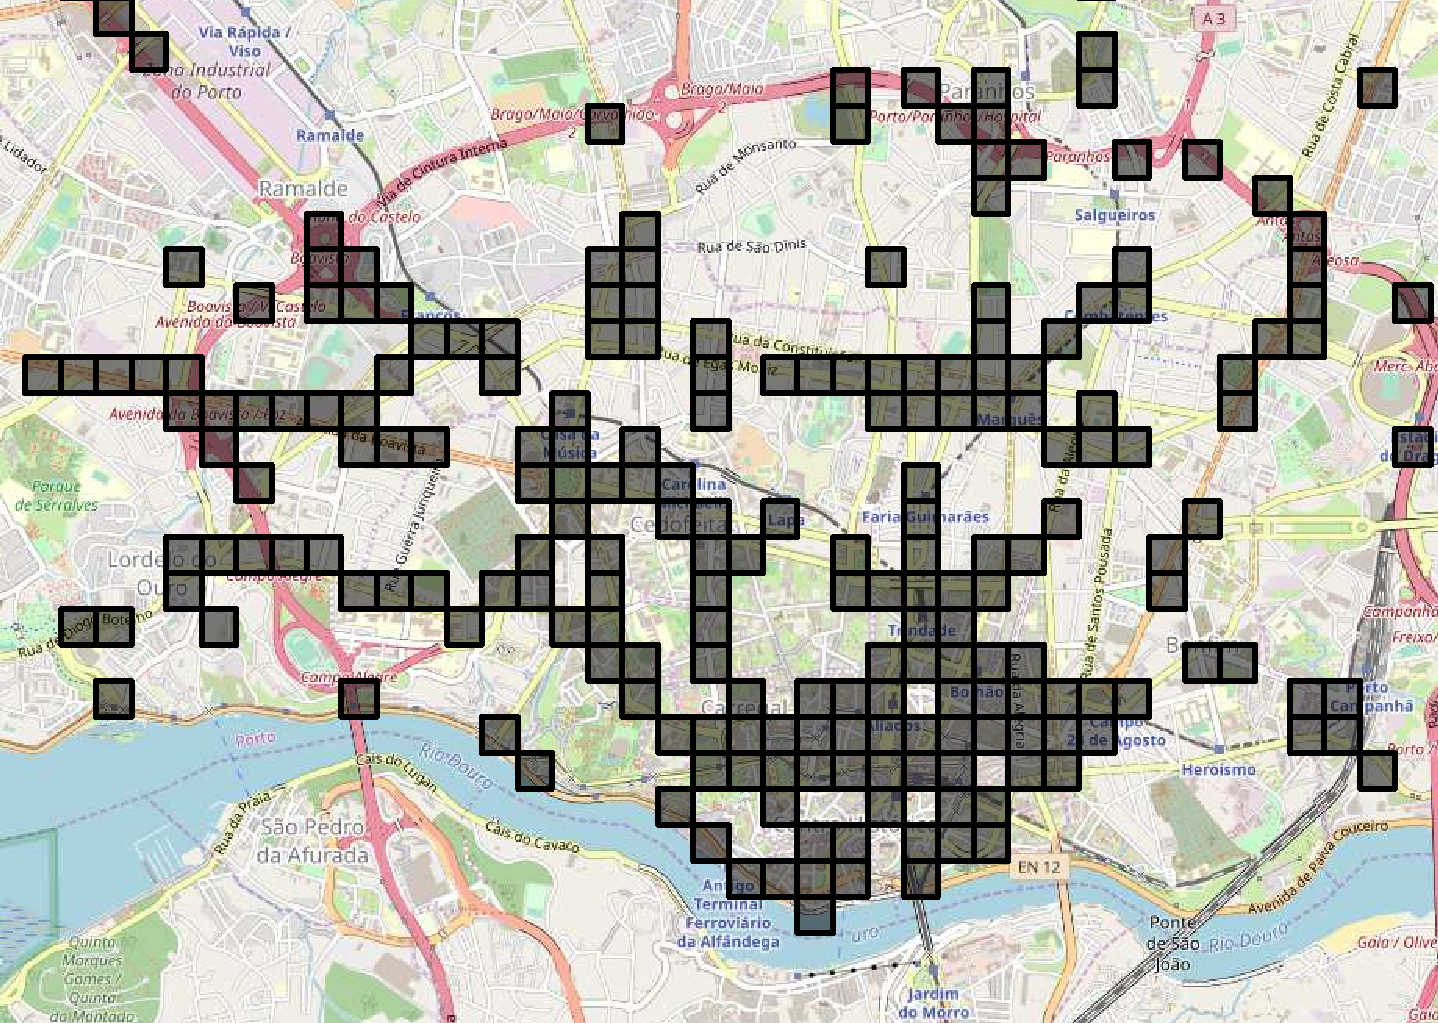
\includegraphics[scale=0.2]{figures/map/grid-init.pdf}
        \caption{Initial set of dense cells}
    \end{subfigure}
    \begin{subfigure}{0.49\textwidth}
        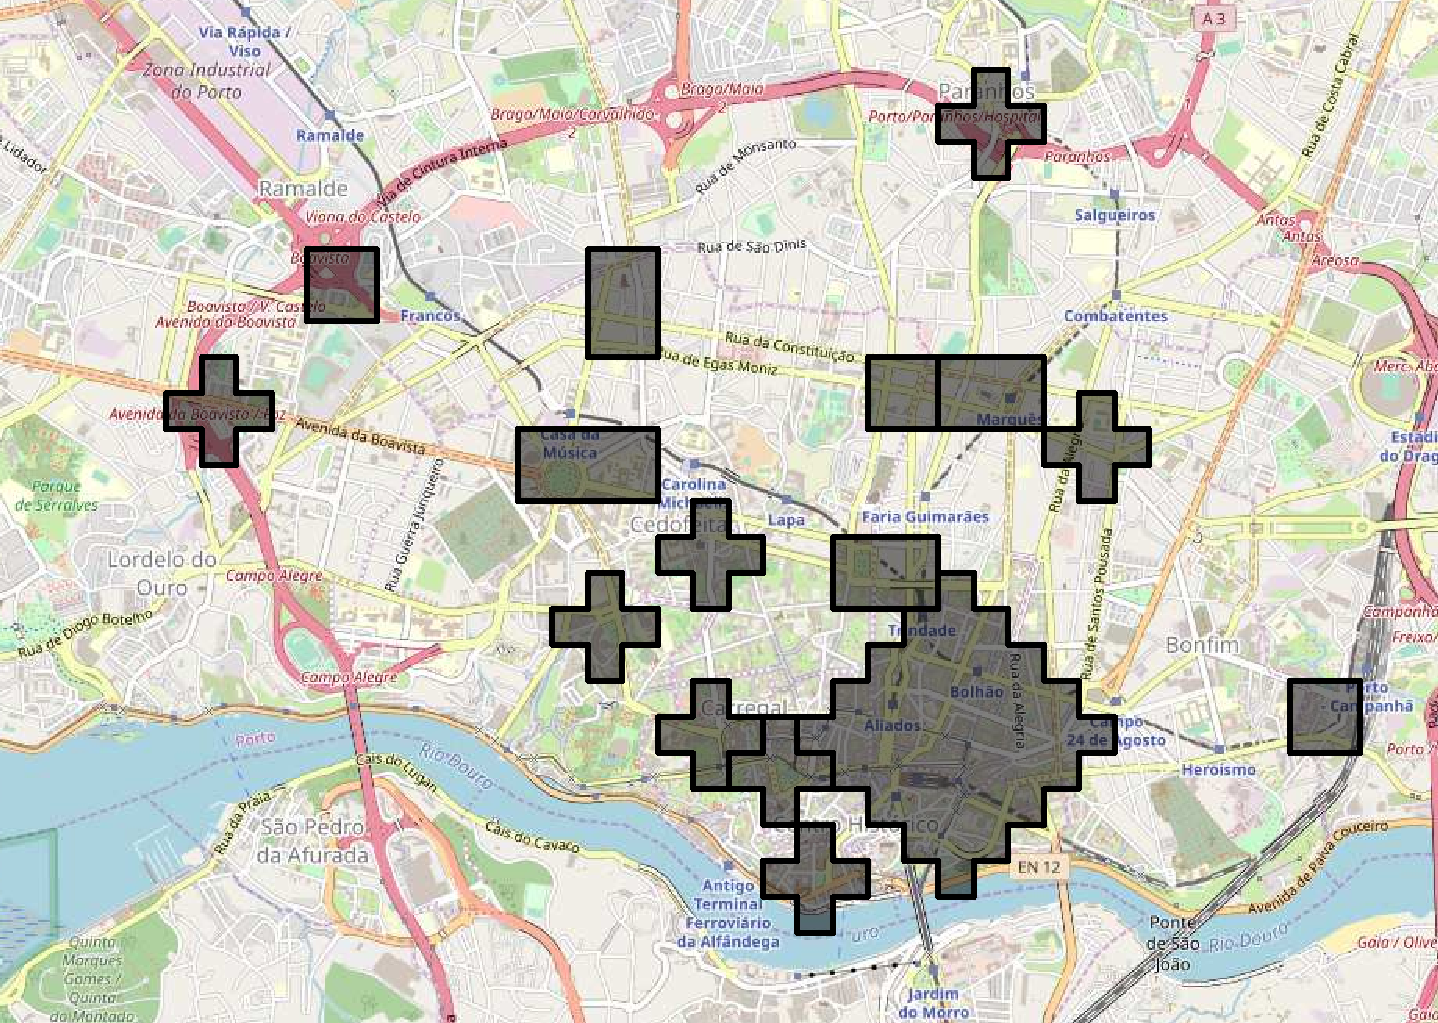
\includegraphics[scale=0.2]{figures/map/grid-ilp.pdf}
        \caption{Solution found by our method}
    \end{subfigure}
\end{figure}
\end{frame}

\section{PopularRegion}

\begin{frame}{Execution of the algorithm}
    \begin{figure}
        \centering
        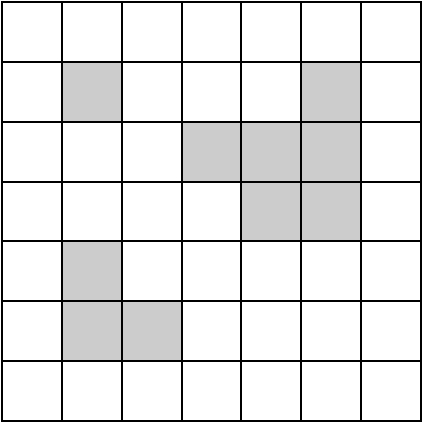
\includegraphics{figures/running-example/running-ex-init.pdf}
    \end{figure}
    \fullcite{giannotti2007trajectory}
\end{frame}

\newcounter{loop}
\forloop{loop}{1}{\value{loop}<8}{
    \begin{frame}{Execution of the algorithm}
        \begin{figure}
            \centering
            \includegraphics{figures/running-example/PopularRegion/running-ex-pp-\arabic{loop}.pdf}
        \end{figure}
        \fullcite{giannotti2007trajectory}
    \end{frame}
}

\begin{frame}{Result of the algorithm}
\begin{figure}
    \begin{subfigure}{0.49\textwidth}
        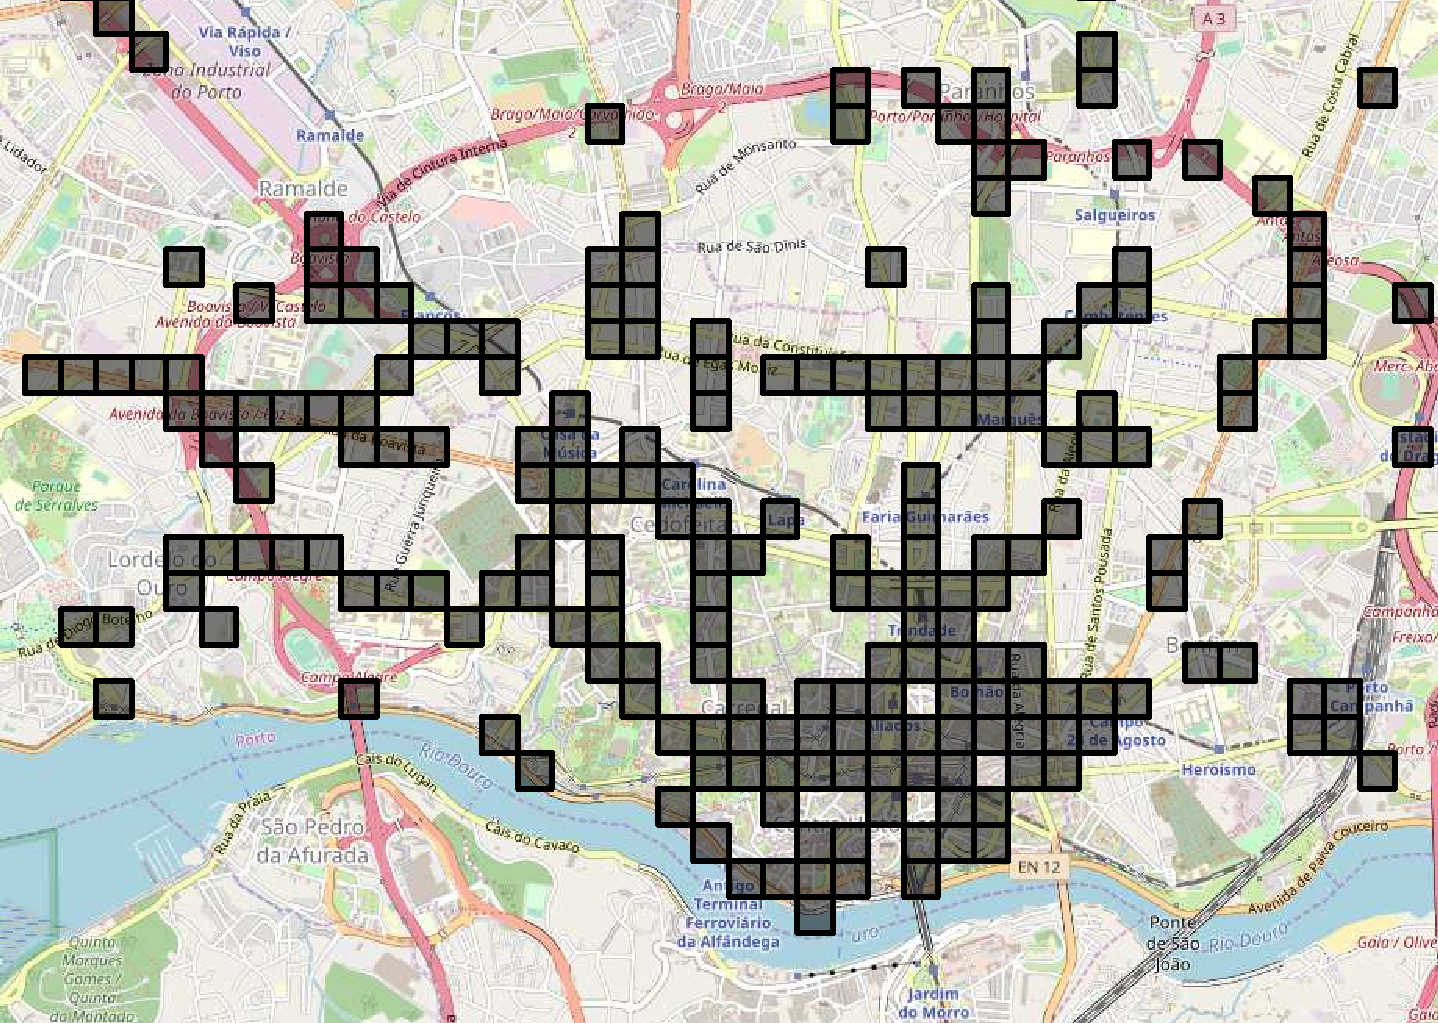
\includegraphics[scale=0.2]{figures/map/grid-init.pdf}
        \caption{Initial set of dense cells}
    \end{subfigure}
    \begin{subfigure}{0.49\textwidth}
        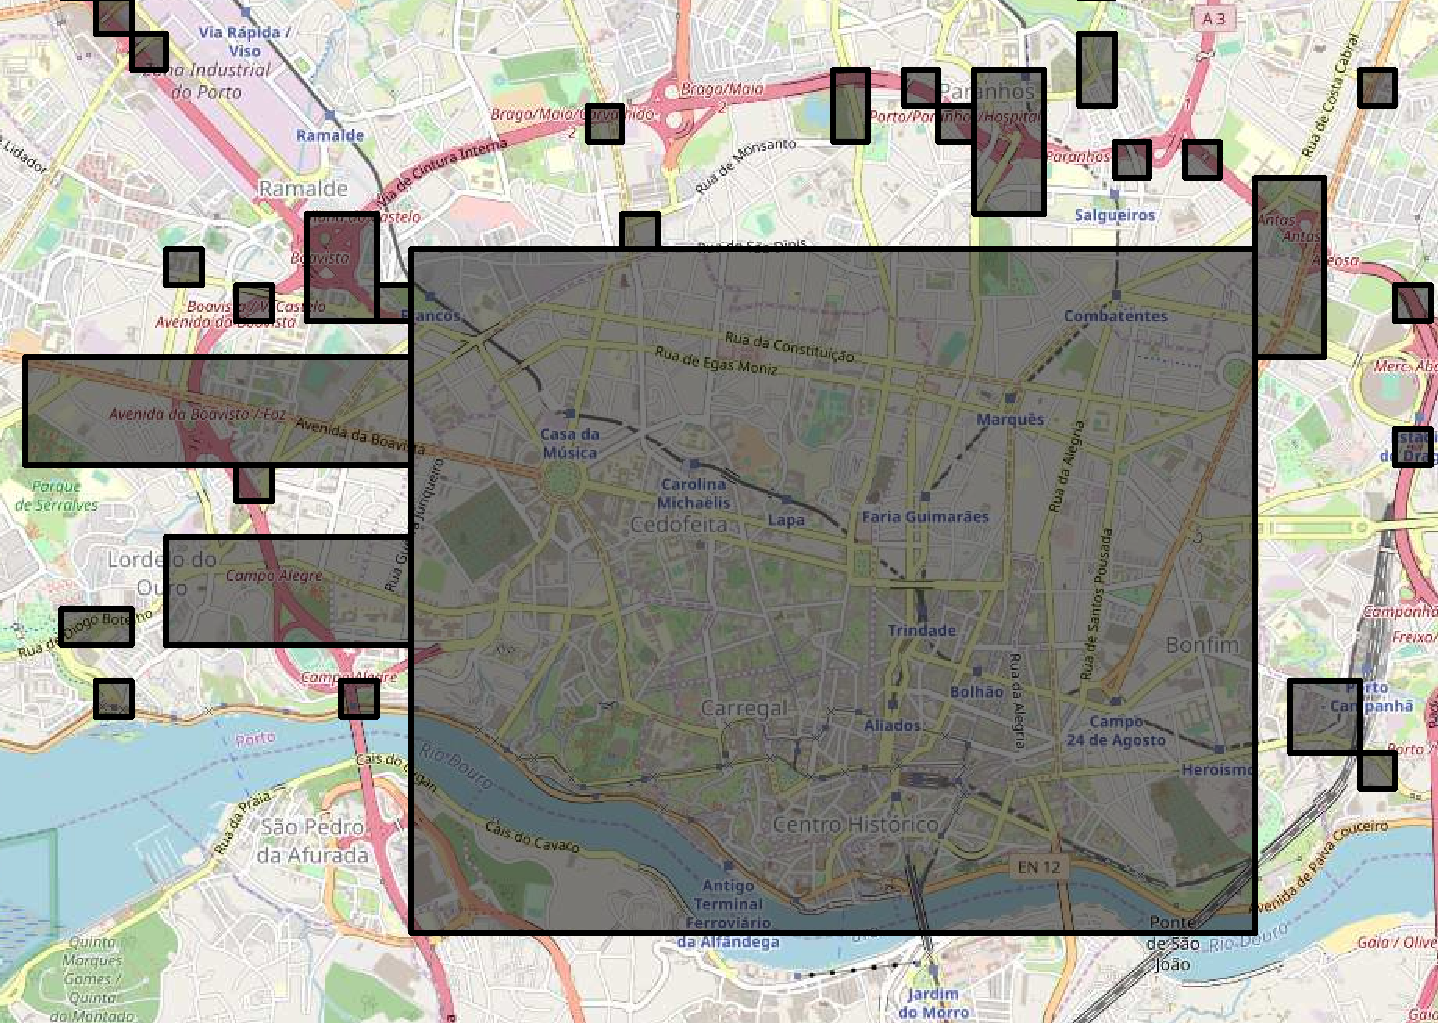
\includegraphics[scale=0.2]{figures/map/grid-pp.pdf}
        \caption{Solution with $5\%$ min average density}
    \end{subfigure}
\end{figure}
\end{frame}

\begin{frame}{Advantages and disadvantages}
    \begin{itemize}
        \item Scalable
        \item Intuitive and good results for most configurations
    \end{itemize}
    But...
    \begin{itemize}
        \item No formalization of the output
        \item Only rectangular regions
        \item Does not easily accept background knowledge
        \item Easy to create pathological input
    \end{itemize}
\end{frame}

\section{Our method}

\begin{frame}{ROIs as an encoder}

\begin{columns}[T, onlytextwidth]
    \column{.5\textwidth}
    \begin{itemize}
        \item The ROIs encode the dense status of the cells
        \item Example of encoding with two rectangles
        \begin{itemize}
            \item 1 dense cells is not covered
            \item 4 non-dense cells are covered
            \item The encoding makes 5 errors
        \end{itemize}
        \item We prefer encoding with fewer errors
    \end{itemize}
    
    \column{.5\textwidth}
    \begin{figure}
        \centering
        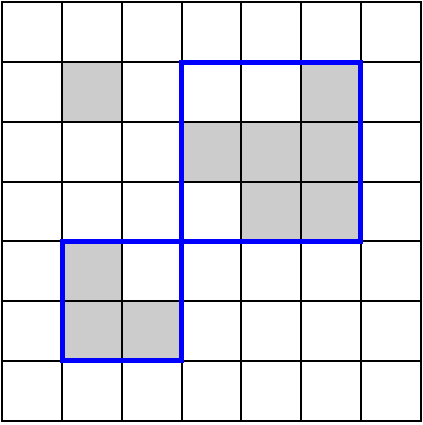
\includegraphics[scale=0.5]{figures/running-example/ILP/running-ex-ilp1.pdf}
    \end{figure}
\end{columns}

\end{frame}

\begin{frame}{Formalization of the problem (1)}
Some notations:
    \begin{itemize}
        \item Let $\mathcal{G}$ be the grid, $\mathcal{G}^*$ the set of dense cells, $\mathcal{S}$ a set of candidates and $\theta$ the minimum density threshold
        \item $d_i$ (resp. $u_i$) is the number of dense (resp. non-dense) cells covered by the candidate $R_i \in \mathcal{S}$
        \item $K$ is the number of ROIs we want to find
    \end{itemize}
\end{frame}

\begin{frame}{A first optimization model}
\begin{IEEEeqnarray*}{r;l;l'l} %note: one extra col to add space at the right
    \IEEEeqnarraymulticol{4}{l}{\mbox{minimize}\ \overbrace{|\mathcal{G}^*| + \sum_{R_i \in \mathcal{S}} x_i \cdot \underbrace{(u_i-d_i)}_{\text{errors of the candidate}}}^{\text{errors of the model}} \label{eq:opti-base}} \label{eq:ext-base2}\\
    \IEEEeqnarraymulticol{4}{l}{\mbox{subject to}}\nonumber\\
    \textstyle\sum_{R_i \in \mathcal{S}} x_i &\leq & K  \label{eq:constr-K}\\
    \textstyle\sum_{R_i \in \mathcal{S} \mid c \in R_i} x_i & \leq & 1 & \forall c \in \mathcal{G} \label{eq:constr-overlap} \\
    x_i & \in & \{0,1\} & \forall R_i \in \mathcal{S} \label{eq:constr-xi}
\end{IEEEeqnarray*}

\end{frame}

\begin{frame}{Formalization of the problem (2)}
    In practice how to set the $K$? Use the Minimum Description Length Principle!
    \begin{itemize}
        \item Let $Sol \subseteq \mathcal{S}$ be a valid selection of candidates
        \item Length of the errors ($2$ integers per cell):
            $$L(\mathcal{G}\mid Sol) = 2(|\mathcal{G}^*| + \sum_{R_i \in Sol} (u_i - d_i))$$
        \item Length of the model: $$L(Sol) = \sum_{R_i \in Sol} size(R_i)$$
        \item Minimum Description Length principle says that the best solution is:
            \begin{equation*}
                \argmin_{Sol \in \mathcal{S}} L(\mathcal{G} \mid Sol) + L(Sol) = 2|\mathcal{G}^*| + \sum_{R_i \in Sol} (2(u_i - d_i) + size(R_i))
            \end{equation*}
    \end{itemize}
\end{frame}

\begin{frame}{The final optimization model}

    \begin{IEEEeqnarray*}{r;l;l'l} %note: one extra col to add space at the right
        \IEEEeqnarraymulticol{4}{l}{\mbox{minimize}\ \sum_{R_i \in \mathcal{S}} x_i \cdot \overbrace{\left(2(u_i-d_i)+size(R_i)\right)}^{\text{Contribution to the description length}}} \label{eq:extended-opti}\\
        \IEEEeqnarraymulticol{4}{l}{\mbox{subject to}}\nonumber\\
        \textstyle\sum_{R_i \in \mathcal{S} \mid c \in R_i} x_i & \leq & 1 & \forall c \in \mathcal{G} \label{eq:extended-ctr} \\
        x_i & \in & \{0,1\} & \forall R_i \in \mathcal{S} \label{eq:extended-integer}
    \end{IEEEeqnarray*}
\end{frame}

\begin{frame}{Example}

    \begin{columns}[T, onlytextwidth]
        \column{.5\textwidth}
            \begin{itemize}
                \item $L(\mathcal{S}) = 4 + 4 = 8$
                \item $L(\mathcal{G} \mid \mathcal{S}) = 2\cdot (4 + 1) = 10$
                \item Total length of this model is $8 + 10 = 18$
            \end{itemize}

        \begin{figure}
            \centering
            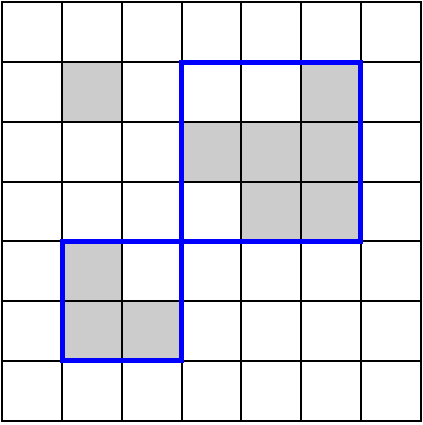
\includegraphics[scale=0.5]{figures/running-example/MDL/example-1.pdf}
        \end{figure}

        \column{.5\textwidth}

            \begin{itemize}
                \item $L(\mathcal{S}) = 4 + 4 = 8$
                \item $L(\mathcal{G} \mid \mathcal{S}) = 2\cdot (2 + 2) = 8$
                \item Total length of this model is $8 + 8 = 16$
            \end{itemize}

        \begin{figure}
            \centering
            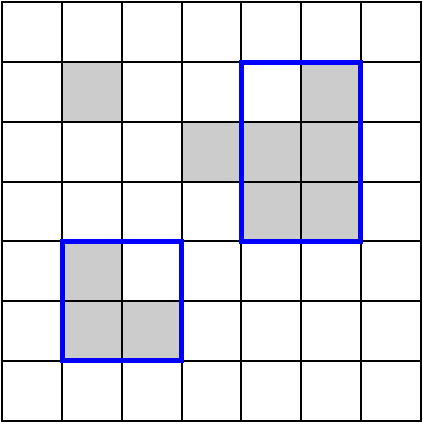
\includegraphics[scale=0.5]{figures/running-example/MDL/example-2.pdf}
        \end{figure}
    \end{columns}
\end{frame}

\begin{frame}{Example with circles}

    \begin{columns}[T, onlytextwidth]
        \column{.5\textwidth}
            \begin{itemize}
                \item $L(\mathcal{S}) = 4 + 4 = 8$
                \item $L(\mathcal{G} \mid \mathcal{S}) = 2\cdot (4 + 1) = 10$
                \item Total length of this model is $8 + 10 = 18$
            \end{itemize}

        \begin{figure}
            \centering
            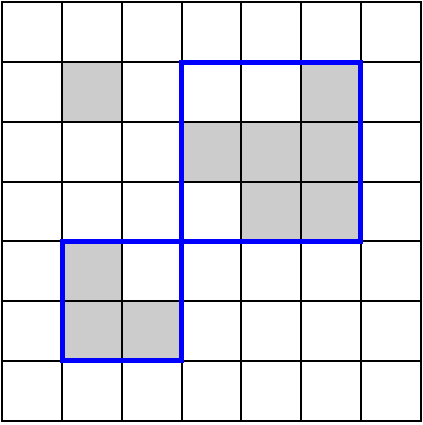
\includegraphics[scale=0.5]{figures/running-example/MDL/example-1.pdf}
        \end{figure}

        \column{.5\textwidth}

            \begin{itemize}
                \item $L(\mathcal{S}) = 4 + 3 = 7$
                \item $L(\mathcal{G} \mid \mathcal{S}) = 2\cdot (2 + 3) = 10$
                \item Total length of this model is $7 + 10 = 17$
            \end{itemize}

        \begin{figure}
            \centering
            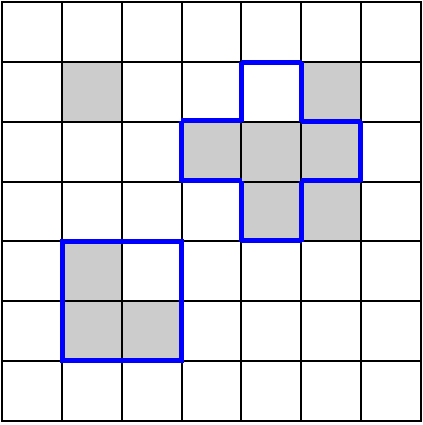
\includegraphics[scale=0.5]{figures/running-example/MDL/example-3.pdf}
        \end{figure}
    \end{columns}
\end{frame}

\begin{frame}{The full method}
    \begin{enumerate}
        \item Generate the set of candidates $\mathcal{S}$ (e.g. enumerate all distinct
            rectangle on the grid)
            \begin{itemize}
                \item Candidate can have any shape
                \item Compute their contribution to the description length
                \item Apply \emph{intra-ROI} constraints to filter the candidate set
            \end{itemize}
        \item Solve the optimization model
            \begin{itemize}
                \item Model \emph{inter-ROI} constraints with linear constraints in the ILP
                \item Solve the ILP, the binary decision variables give the set of ROIs
            \end{itemize}
    \end{enumerate}
\end{frame}


\section{Experiments}

\begin{frame}{Setup}
    \begin{itemize}
        \item Two versions of our method
            \begin{itemize}
                \item With only rectangular regions
                \item With rectangular and circular regions
            \end{itemize}
        \item Showing results on Kaggle taxis dataset ($\approx$1.6 million trajectories)
        \item Comparing with PopularRegion\footfullcite{giannotti2007trajectory} and OPTICS\footfullcite{ankerst1999optics} (when clustering the dense cells)
    \end{itemize}
\end{frame}

\begin{frame}{Execution time}
\begin{table}[!htb]
\centering
{\resizebox{\linewidth}{!}{
\setlength{\tabcolsep}{7pt}
\begin{tabular}{lllllll}
\toprule
Minimum density threshold & \multicolumn{3}{c}{2\%} & \multicolumn{3}{c}{5\%} \\
\cmidrule(lr){2-4} \cmidrule(l){5-7}
Grid side size            & 100 & 150 & 200           & 100 & 150 & 200 \\
\midrule
Number of dense cells ($|\mathcal{G}^*|$) & 571 & 597 & 537 & 230 & 178 & 137 \\
\addlinespace 
Number of ILP candidates                  & 23 814 & 7 779 & 3 399 & 2 880 & 1 232 & 434 \\
ILP optimization time (s)                 & 4.328 & 0.464 & 0.109 & 0.113 & 0.044 & 0.029 \\ 
\addlinespace 
\emph{PopularRegion} run time (s)       & 0.003 & 0.005 & 0.006 & 0.002 & 0.003 & 0.004 \\
\addlinespace 
OPTICS run time (s)                          & 0.209 & 0.222 & 0.200 & 0.084 & 0.065 & 0.051 \\
\bottomrule
\end{tabular}%
}}
\end{table}
\end{frame}

\begin{frame}{Description Length}
    \begin{itemize}
        \item For high density threshold, number of errors becomes similar
        \item ILP-based methods produce smaller models
        \item Overall the Description Length is inferior for ILP-based methods
    \end{itemize}
    \begin{columns}[T, onlytextwidth]

        \column{.5\textwidth}
        \begin{figure}
            \centering
            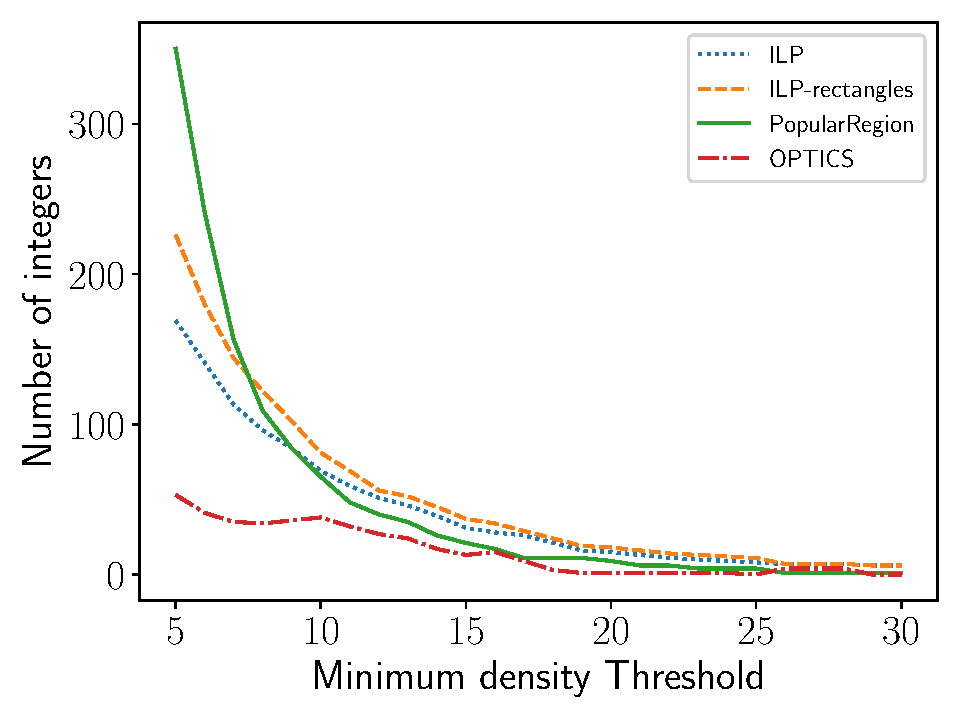
\includegraphics[scale=0.3]{figures/results/error-rate.pdf}
            \caption{Encoding of the errors}
        \end{figure}

        \column{.5\textwidth}
        \begin{figure}
            \centering
            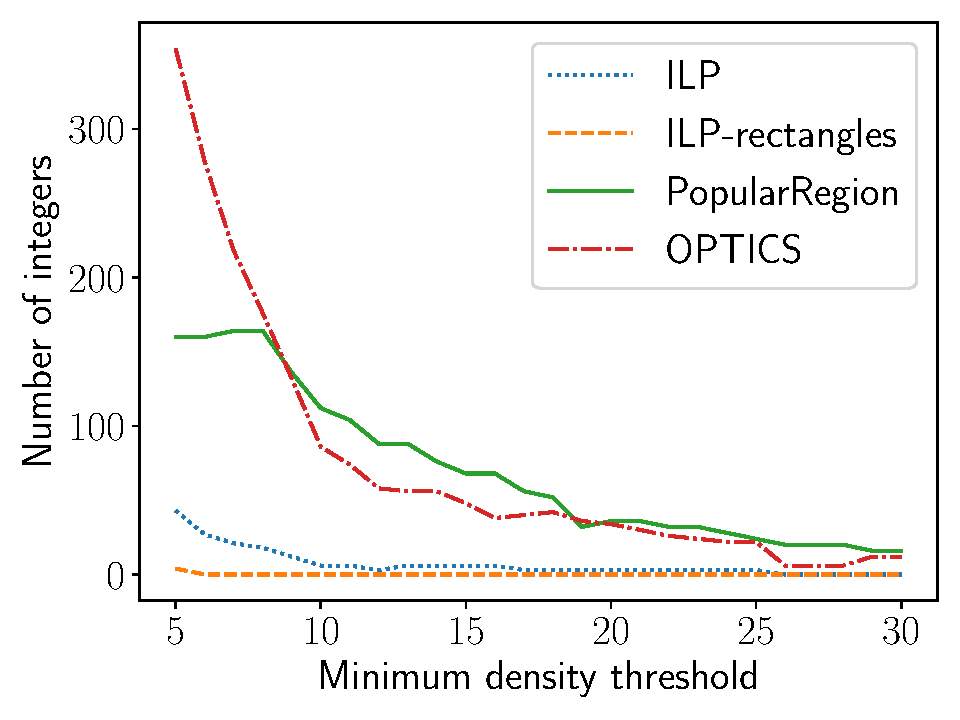
\includegraphics[scale=0.3]{figures/results/model-length.pdf}
            \caption{Encoding fo the models}
        \end{figure}
    \end{columns}
\end{frame}

\begin{frame}{Robustness to noise}
    \begin{itemize}
        \item Start from a $100 \times 100$ grid
        \item Move every element of the trajectories to a new cell with a probability $p$
        \item Choose the new cell randomly in a square of size $10$ around the initial cell
        \item Compute the solution from the noisy grid and compute the \emph{precision, recall} and \emph{F1-measure}.

    \end{itemize}
    \begin{columns}[T, onlytextwidth]

        \column{.5\textwidth}
        \begin{figure}
            \centering
            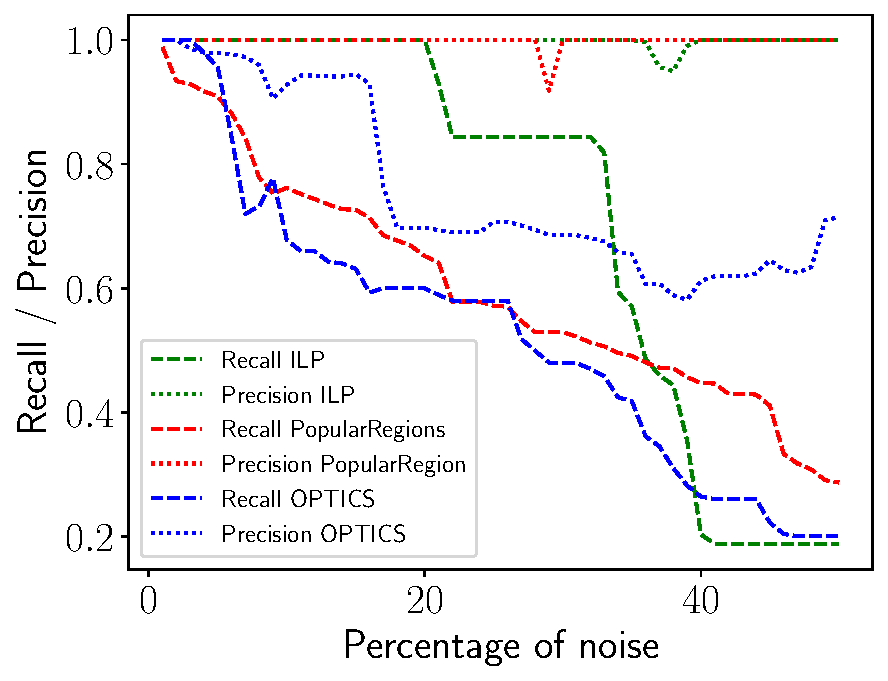
\includegraphics[scale=0.3]{figures/results/recall-precision.pdf}
            \caption{Recall and precision}
        \end{figure}

        \column{.5\textwidth}
        \begin{figure}
            \centering
            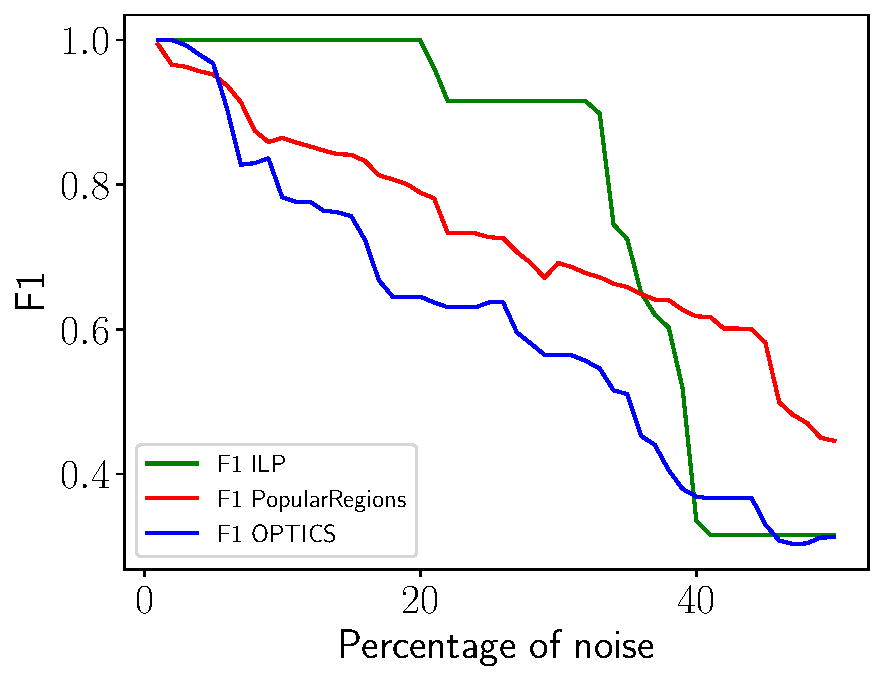
\includegraphics[scale=0.3]{figures/results/f1.pdf}
            \caption{F1-measure}
        \end{figure}
    \end{columns}
\end{frame}

\begin{frame}{Conclusion and Future work}
    What we did:
    \begin{itemize}
        \item We propose an optimization model to find $K$ ROIs from trajectory data
        \item Our method is more flexible than specific method since it accepts a wide range of constraints
        \item The runtime of the ILP becomes reasonable as long as there is not too much candidates
        \item Everything is Open Source, see \url{https://github.com/AlexandreDubray/mining-roi}
    \end{itemize}
    The next steps:
    \begin{itemize}
        \item Get rid of the grid
        \item Use the density information (instead of just dense/not dense)
        \item Provide support for more complex constraints
    \end{itemize}
\end{frame}

\end{document}
